\chapter{Linear Maps, Kernals and Range}

\begin{definition}
	Let $U$ and $V$ be vector spaces over the same field $F$. A mapping $T:U \rightarrow V$ is linear if 	$ \forall u_1, u_2 \in U, \forall \lambda \in F$ 
	\begin{center}
 		$T(u_1 + u_2) = T(u_1) + T(u_2)$\\ 
 		$T(\lambda u_1) = \lambda T(u_1)$
	\end{center}
	
\end{definition}

The set of all linear mappings from $U \rightarrow V$ is denoted by $\mathcal{L}(U,V)$. If $U=V$, then linear mappings are denoted by $\mathcal{L}(U)$, which is a set of linear mappings from a set onto itself. \\ 

\textbf{Examples}
\begin{itemize}
	\item $T: \mathcal{C}[a, b] \rightarrow \Re$, $f \rightarrow \int_{a}^{b} f(x) dx$. Integration is linear operator since it does not matter whether you add two functions and then integrate or vice versa. Also, we can pull out scalar multiples out of the integrals. 
	\item $D: \mathcal{C}^{\infty} [a, b] \rightarrow \mathcal{C}^{\infty} [a, b]$, $f \rightarrow f'$. The derivative of the sum of functions is the same as taking the sum and then derivatves. \\
\end{itemize}

\begin{definition}
	$T \in \mathcal{L}(U, V)$. Then the kernal of $T$ (null space) is defined as : 
	\begin{center}
		$ker(T) := null(T) := \{u \in U | Tu = 0\}$
	\end{center}
	
\end{definition}

\begin{proposition}
	$ker(T)$ is a subspace of $U$.
\end{proposition}

$T$ is injective iff $ker(T) = \{0\}$. Means if we take two input points in the input space then they are always mapped to different points in the output space. 
So 0 is always an element in the kernal since a linear map always maps 0 to 0. Thus the kernal is never empty. The smallest kernal of any vector space is just the 0 vector. 

\begin{definition}
	The range of $T$ (image of $T$) is defined as: 
	\begin{center}
		$range(T) := Image(T) := \{Tu | u \in U\}$
	\end{center}
\end{definition}

\begin{proposition}
	The range is always a subspace of $V$
\end{proposition}

$T$ is surjective iff $range(T) = V$

\begin{definition}
	$V' \subset V$ where $V'$ is any set. The pre-image of $V'$ is defined as: 
	\begin{center}
		$T^{-1} (V') := \{u \in U | Tu \in V'\}$
	\end{center} 
\end{definition}

\begin{proposition}
	If $V' \subset V$ is a subspace of V, then $T^{-1}(V')$ is a subspace of $U$.
\end{proposition}

\begin{figure}[h]
	\centering
	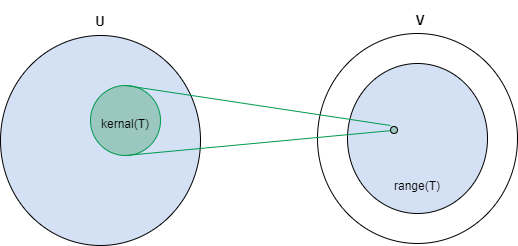
\includegraphics[width=0.5\textheight]{ch-3-img-1}
	\caption{Kernal and range of a $T: U \rightarrow V$}
\end{figure}

We can see in the figure above that a part of $U$ which is mapped to 0 is known as the kernal of tha map $T$. The range lives in $V$ and the kernal lives in $U$. 

\begin{theorem}
	Let $V$ be finite dimensionalm $W$ be any vector space and $T \in \mathcal{L}(V,W)$. Let $u_1,...,u_n$ be a basis of $ker(T) \subset V$. Let $w_1,...,w_m$ be a basis of the $range(T) \subset W$. Then $u_1,...,u_n$, $T^{-1}(w_1),...,T^{-1}(w_m)$ forms a basis of $V$. In particular , $dim(V) = dim(ker(T)) + dim(range(T))$
\end{theorem}

\begin{proof}
	Denote $T^{-1}(w_1) := z_1,...,T^{-1}(w_m) := z_m$. If $\{u_1,...u_n,z_1,...z_m\}$ for a basis of $V$, then they must span the whole space $V$ and be linearly independent. Let's do each step by step. \\
	Step 1: Prove that $V \subset span\{u_1,...u_n,z_1,...z_m\}$ \\ 
	Let $v \in V$, and $Tv \in range(T)$. Since we know the basis of $range(T)$,
	\begin{align*}
		\exists \lambda_1,...,\lambda_m: Tv &= \lambda_1 w_1 + ... + \lambda_m w_m \\
											&= \lambda_1 T(z_1) + ... + \lambda_m T(z_m) \\
											&= T(\lambda_1 z_1) + ... + T(\lambda_m z_m)
	\end{align*}
$ \implies Tv - T(\lambda_1z_1 + ... + \lambda_mz_m) = T(v - (\lambda_1z_1 + ... + \lambda_mz_m)) =  0$  \\
$\implies (v - (\lambda_1z_1 + ... + \lambda_mz_m)) \in kernal(T)$ since this vector is mapped to 0 by the linear mapping. Since we also know the basis of the kernal any vector in the kernal can be written as: 
\begin{align*}
(v - (\lambda_1z_1 + ... + \lambda_mz_m)) &= \mu_1 u_1 + ... + \mu_n u_n \\ 
v &= \lambda_1 z_1 + ... + \lambda_m z_m + \mu_1 u_1 + ... + \mu_n u_n
\end{align*}
Step 2 : Prove that $u_1,...,u_n, z_1,...,z_m$ are linearly independent. \\ 
Assume that $\mu_1 u_1 + ... \mu_n u_n + \lambda_1 z_1 + ... + \lambda_m z_m  = 0$ \\
If these vectors are linearly independent then all the coefficients will simultaneously go to zero. 
\begin{align*}
	\lambda_1 w_1 + ... + \lambda_m w_m &= \lambda_1 T(z_1) + ... + \lambda_m T(z_m) \\
	&= \lambda_1 T(z_1) + ... + \lambda_m T(z_m) + \mu_1 T(u_1) + ... + \mu_n T(u_n) \\ 
	&= T(\lambda_1 z_1 + ... \lambda_m z_m + \mu_1 u_1 + ... + \mu_n u_n) = T(0) = 0
\end{align*}
We can add $ \mu_1 T(u_1) + ... + \mu_n T(u_n)$ to the expression since it goes to zero by definition of a kernal. Everything inside the operator is zero due to the assumption at the beginning of step 2. 
Since $\lambda_1 w_1 + ... + \lambda_m w_m = 0$ and $w_1,...,w_m$ is a basis 
$\implies \lambda_1 = ... = \lambda_m = 0$ \\
Now $\mu_1 u_1 + ... + \mu_n u_n = 0$ since we have already proved the other half of the assumption to be zero. Since $u_1,...,u_n$ is the basis of the kernal $\implies \mu_1=...\mu_n=0$.
\end{proof}

\begin{proposition}
	Let $T \in \mathcal{L}(V, W)$ and $V, W$ be finite dimensional, then the following statements are equivalent.
	\begin{itemize}
		\item T is injective
		\item T is surjective
		\item T is bijective
	\end{itemize} 
\end{proposition}

This proposition does not hold in infinite dimensional spaces. 



